\section{Konzept 1}
Das erste Konzept basiert auf der Verwendung von industriellen Partikelgeneratoren und mechanischen Ventilen. Hierbei gibt es zwei M\"{o}glichkeiten den Strom zu erzeugen, die im Folgenden n\"{a}her erl\"{a}utert werden sollen. Der Fokus liegt bei diesen Konzepten auf dem Rohrsystem, da die eigentlichen Bauteile bereits funktionsf\"{a}hig gekauft werden und nur verbaut werden m\"{u}ssen.

\subsection{Aufbau}
Der Versuchsaufbau besteht aus einer Parallelschaltung eines Aerosolgenerators mit einem Ventilator. Der Ventilator erzeugt einen reinen Luftstrom der mit dem Aerosolstrom in das selbe Rohr geleitet wird. In diesem Rohr ist eine Mischvorrichtung installiert, welche aus Luft- und Aerosolstrom eine homogene Mischung erzeugt. Das Rohr endet am Anschluss(\textit{Anschluss 1}) eines 4/2 - Wegeventils (\ref{fig:ventil}). Ein Ausgang des Ventils (\textit{Anschluss 2}) f\"{u}hrt raus in die Umgebungsluft, \textit{Anschluss 4} f\"{u}hrt \"{u}ber einen Adapter direkt an den Einlass des Messger\"{a}tes. Dabei ist es wichtig, darauf zu achten, dass die Verbindung zwischen Ventil und Messger\"{a}t so kurz wie m\"{o}glich gehalten wird um die Totzeit des Systems klein zu halten. Dennoch muss es mindestens so lang sein um einen moderaten Querschnitts\"{u}bergang zu gew\"{a}hrleisten, um Druck- und Partikelverluste zu minimieren. \textit{Anschluss 3} des Ventils ist mit einem weiteren Ventilator verbunden, welcher auch einen reinen Luftstrom erzeugt. Dieser Luftstrom ist f\"{u}r die Nullphase des Messger\"{a}tes gedacht.
\begin{figure}[H]
        \myfloatalign
        {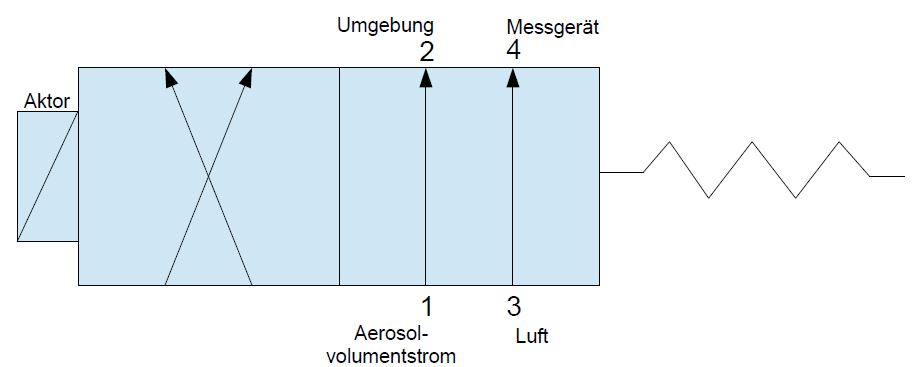
\includegraphics[width=.9\linewidth]{gfx/concepts/ventil_feder.jpg}} \quad
        \caption[Schaltm\"{o}glichkeiten von 4/2-Wegeventilen]
        {Schaltm\"{o}glichkeiten von 4/2-Wegeventilen}
        \label{fig:ventil}
\end{figure}

\newpage

\subsection{Funktionsweise}
Der Aerosolgenerator generiert einen konstanten Partikelmassenstrom mit einstellbaren Partikeleigenschaften wie die Konzentration oder die Gr\"{o}{\ss}enverteilung der Partikel. Zusammen mit der Luft aus dem externen Ventilator kann die Partikelkonzentration zus\"{a}tzlich nochmal reguliert werden und der Aerosolstrom dem angeschlossenen Messger\"{a}t angepasst werden. Die anschlie{\ss}ende Mischvorrichtung sorgt f\"{u}r eine gleichm\"{a}{\ss}ige \"{u}ber den Rohrquerschnitt verteilte Partikelkonzentration sowie eine laminare Str\"{o}mung beim Eintritt in das Ventil. Der Vorteil davon liegt darin, dass manche Messger\"{a}te dem Volumenstrom noch vor dem Passieren der Messkammer einen Schleierstrom (\textit{Sheath-Air}) entnehmen, da dieser abgezweigte Strom bei hohem Konzentrationsgradienten in radialer Richtung zu starken Schwankungen in der Konstanz des Partikelstroms f\"{u}hren kann. Das 4/2 - Wegeventil zeichnet sich durch vier Anschl\"{u}sse und zwei Schaltstellungen aus. Dabei ist in der stabilen Position (\textit{Stellung 0}) \textit{Anschluss 1} direkt mit \textit{Anschluss 2} verbunden. Dementsprechend f\"{u}hrt \textit{Anschluss 3} zu \textit{Anschluss 4}, welcher in das Messger\"{a}t m\"{u}ndet. In der monostabilen Stellung (\textit{Stellung 1}) f\"{u}hrt der Aerosolstrom (\textit{Anschluss 1}) direkt zum Messger\"{a}t (\textit{Anschluss 4}) und der Anschluss des Ventilators (\textit{Anschluss 3}) f\"{u}hrt direkt \"{u}ber \textit{Anschluss 2} in die Umgebungsluft. Das Ventil kann dabei elektronisch oder pneumatisch geschaltet werden. Der extern angetriebene Ventilator treibt Umgebunsluft durch einen Nullfilter zu dem jeweils geschalteten Anschluss. Dabei ist wichtig, dass der Volumenstrom der reinen Luft dem ben\"{o}tigten Volumenstrom des Messger\"{a}tes entspricht. Der Nullfilter sorgt f\"{u}r einen hohen Partikelkonzentrationsunterschied des Messger\"{a}teeinlassstroms zwischen Stellung 0 und Stellung 1 des Ventils.

\subsection{Durchf\"{u}hrung}
Als erstes stellt man den externen Ventilator an \textit{Anschluss 3} auf den Volumenstrom des Messger\"{a}tes ein und schlie{\ss}t das Messger\"{a}t dann \"{u}ber den Adapter an \textit{Anschluss 4} an.\\
Die Vorlaufzeit, also die Zeit bevor das Ventil geschaltet wird, h\"{a}ngt von mehreren Faktoren ab. So hat das Messger\"{a}t eine Einlaufzeit, nach der es erste zuverl\"{a}ssige Ergebnisse liefert. Nach Ablauf dieser Nullzeit wird das Messger\"{a}t weiter mit dem durch den Ventilator angetriebenen Luftvolumenstrom durchstr\"{o}mt. Parallel dazu laufen der Aerosolgenerator und der andere Ventilator, bis sie die gew\"{u}nschten Stromeigenschaften liefern. Diese Laufzeit ist vor allem von der Einstellzeit des Aerosolgenerators abh\"{a}ngig, welche die Anpassung eines Ausgangsparameters auf eine \"{A}nderung eines Eingangsparameters beschreibt. Nachdem die Voraussetzungen eines eingelaufenen Messger\"{a}tes und eines konstanten Aerosolstroms erf\"{u}llt sind, kann das Ventil geschaltet werden und der korrigierte Verlauf der Sprungantwort mit dem Eingangssignal verglichen werden. Die Korrektur betrifft hierbei die Berechnung der systematischen Totzeit des Versuchsaufbaus, welche sich aus der Schaltzeit des Ventils und der Zeit, welche die Partikelfront braucht um den Messger\"{a}teeinlass zu erreichen, zusammensetzt.

\subsection{Variation: Konzept 2}
Der Aufbau des ersten Konzeptes l\"{a}sst sich stark vereinfachen, wenn Messger\"{a}te benutzt werden, welche mit geringen Volumenstr\"{o}men arbeiten. Der geringe Volumenstrom ist alleine durch den Aerosolgenerator ohne einen externen Ventilator erreichbar. Somit ist auch die Mischvorrichtung zur Homogenisierung \"{u}berfl\"{u}ssig, was zu einem einfacher zu berechnenden Aufbau f\"{u}hrt. Voraussetzung ist, wie schon im oberen Konzept, dass das benutzte Messger\"{a}t durch externe Pumpen betrieben werden kann. Dies ist zum Beispiel beim \textit{OPS 3330} der Fall, somit eignet sich diese Variation des ersten Konzepts vor allem f\"{u}r dieses Messger\"{a}t. Die anderen Teill\"{o}sungen und die Durchf\"{u}hrung dieser Variante sind analog zu erstem Konzept.
\begin{figure}[H]
        \myfloatalign
        \subfloat[Konzept 1 mit Luftmischer]
        {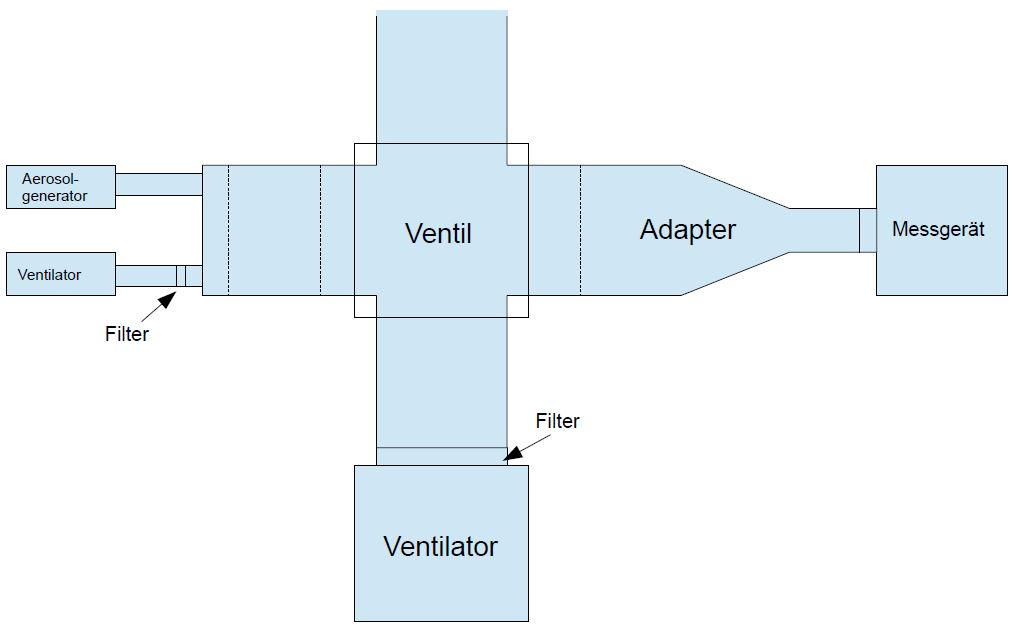
\includegraphics[width=.45\linewidth]{gfx/concepts/Konzept_1.jpg}} \quad
        \subfloat[Variation ohne Luftbeimischung]
        {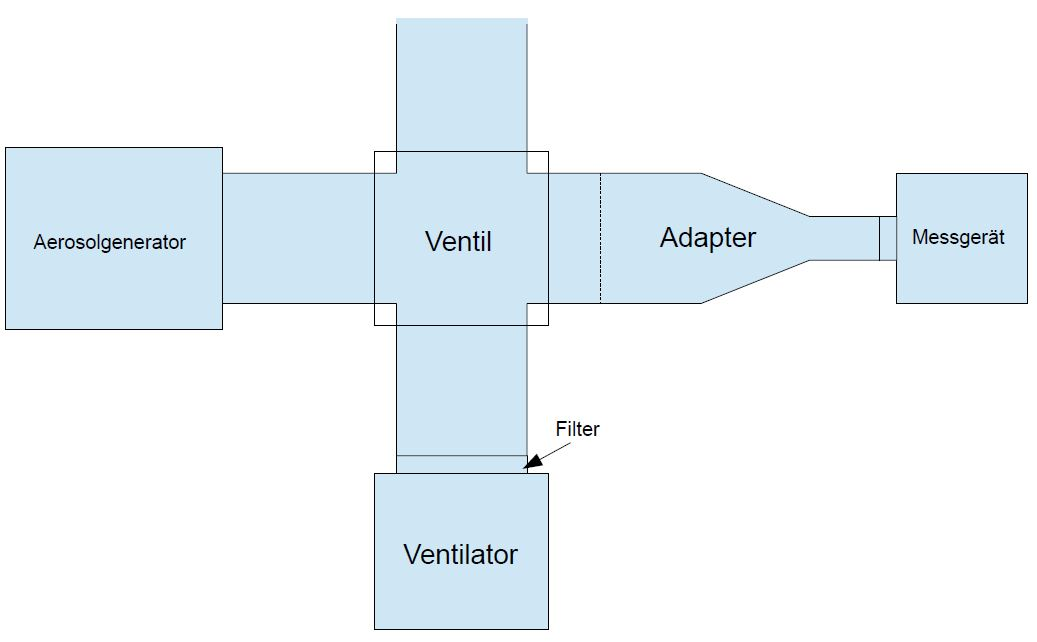
\includegraphics[width=.45\linewidth]{gfx/concepts/Konzept_2.jpg}} 
        \caption[Konzepte 1 und 2 (Vereinfachung)]
        {Konzepte 1 und 2 (Vereinfachung)}
        \label{fig:concepts_1_2}
\end{figure}

